\subsubsection{Zone Calculation}\label{alg:zon_calculation}
The graph colouring algorithm used by the MAPC server to determine occupied zones is described in detail in the MAPC 2014 scenario description~\cite{ahlbrecht_mapc_2014} and will not be explained again here.
To position themselves in an optimally-scoring way, agents could run the same algorithm locally to calculate the agent placement that will lead to the highest total sum of zone scores in each step by trying every possible permutation.
However, the number of ways to place $n$ agents on $k$ nodes is $C \left (n+r-1,r-1\right )= \frac{\left(n+r-1 \right )!}{n!\left(r-1 \right )!}$, a number that increases rapidly with $n$ and $k$.
In particular, there are $C \left (28+600-1,600-1 \right ) =\num{3.7463887025070038e+48}$ ways to place 28 agents on 600 nodes, which were the numbers used in the 2014 competition---far too many to calculate in real-time.

Finding an algorithm that calculates high-scoring zones in a limited computation time is one of the major challenges of the MAPC competition.
Our team developed a heuristic algorithm to calculating zones that will be explained below.
The goal is to find, for every node in the graph, a placement of agents around that node such that:
\begin{itemize}
  \item All of the centre node's one-hop neighbours (those nodes directly connected to the center node through a single edge) will be included in the zone.
  \item Agents can only be placed on the centre node's two-hop neighbours, which are those nodes that can be reached from the centre node through a minimum of two edges.
  \item The constructed zone's value per agent should be high.
        Ideally, it would be maximal, but the heuristic we use doesn't guarantee this.
\end{itemize}
\autoref{fig:zones} shows some examples of zones that are found using our heuristic algorithm.
\begin{figure}
  \centering
  \subcaptionbox{This zone was calculated for a centre vertex that only has a degree of 1, i.e.\ that is a leaf vertex.
                 Generally, it is preferable to place an agent on the cut vertex that leads to a leaf vertex rather than the leaf vertex itself, as this would establish at least a zone of equal size, and possibly larger.
                 \label{fig:zones_1}}[.49\linewidth]{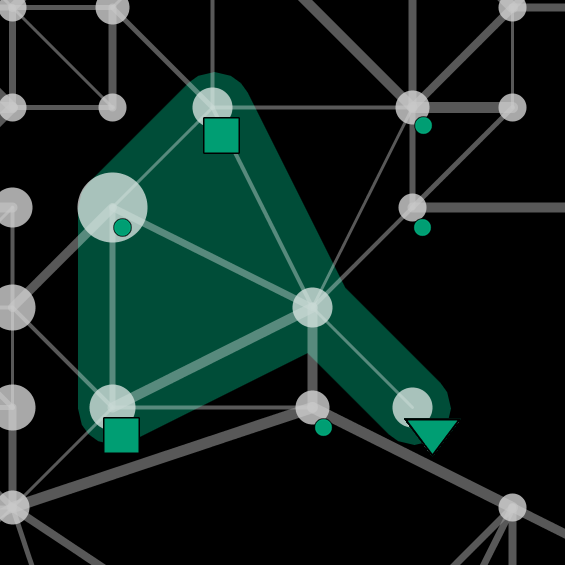
\includegraphics[width=.49\linewidth]{images/zone1.png}}
  \subcaptionbox{Here, the centre vertex has a degree of 3, and the calculated zone remains compact with only two additional agents used.
                 A lot of optional agent positions remain.
                 \label{fig:zones_2}}[.49\linewidth]{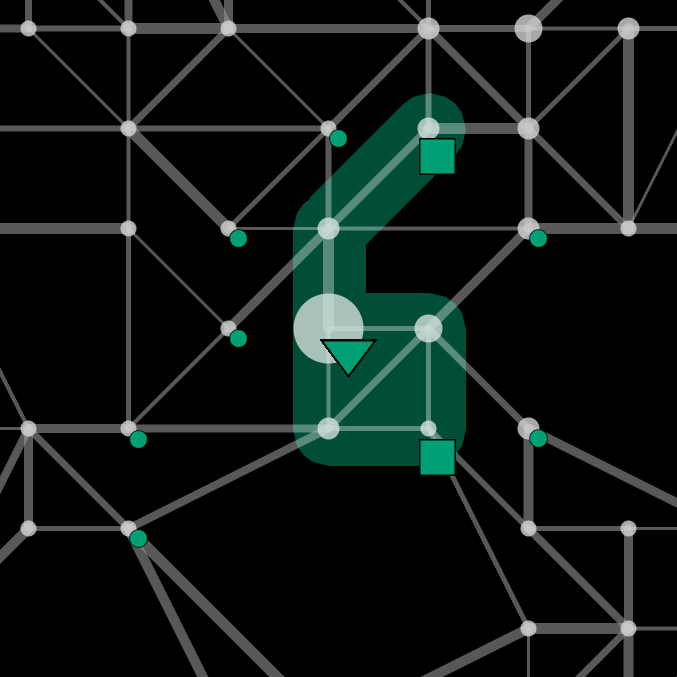
\includegraphics[width=.49\linewidth]{images/zone2.png}}
  \\
  \subcaptionbox{A zone where the centre vertex has a degree of 5, and the zone uses a total of 4 agents.
                 \label{fig:zones_3}}[.49\linewidth]{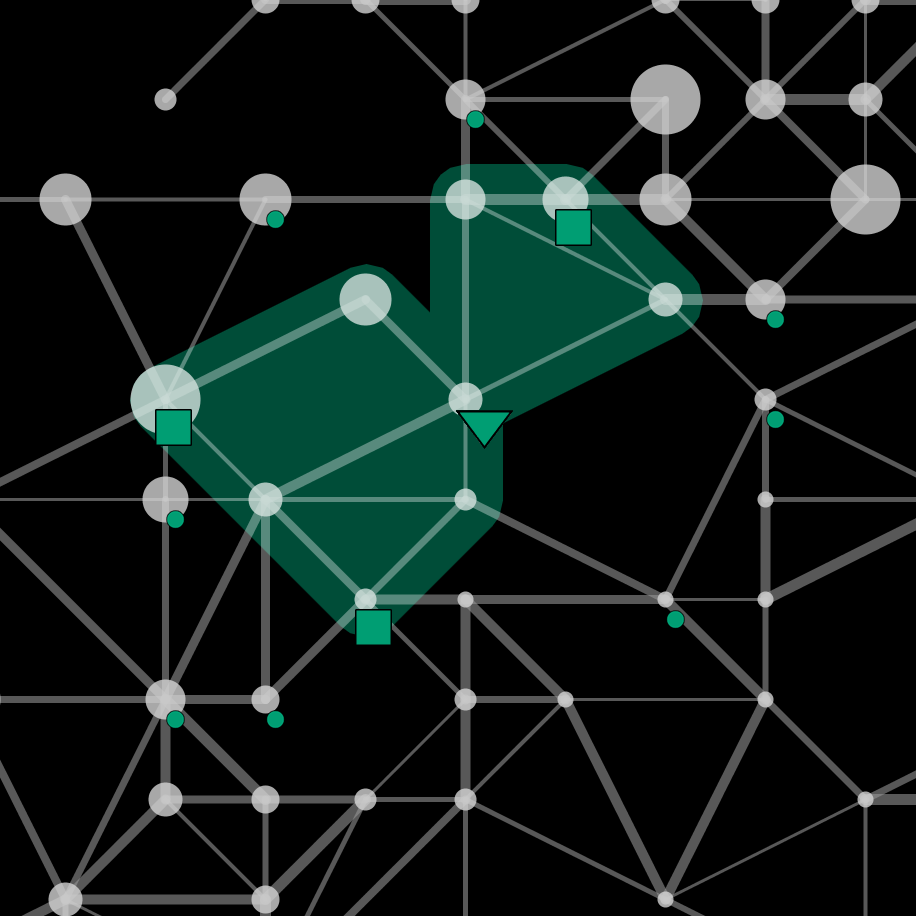
\includegraphics[width=.49\linewidth]{images/zone3.png}}
  \subcaptionbox{A zone where the centre vertex has a degree of 7, and the zone uses a total of 9 agents.
                 \label{fig:zones_4}}[.49\linewidth]{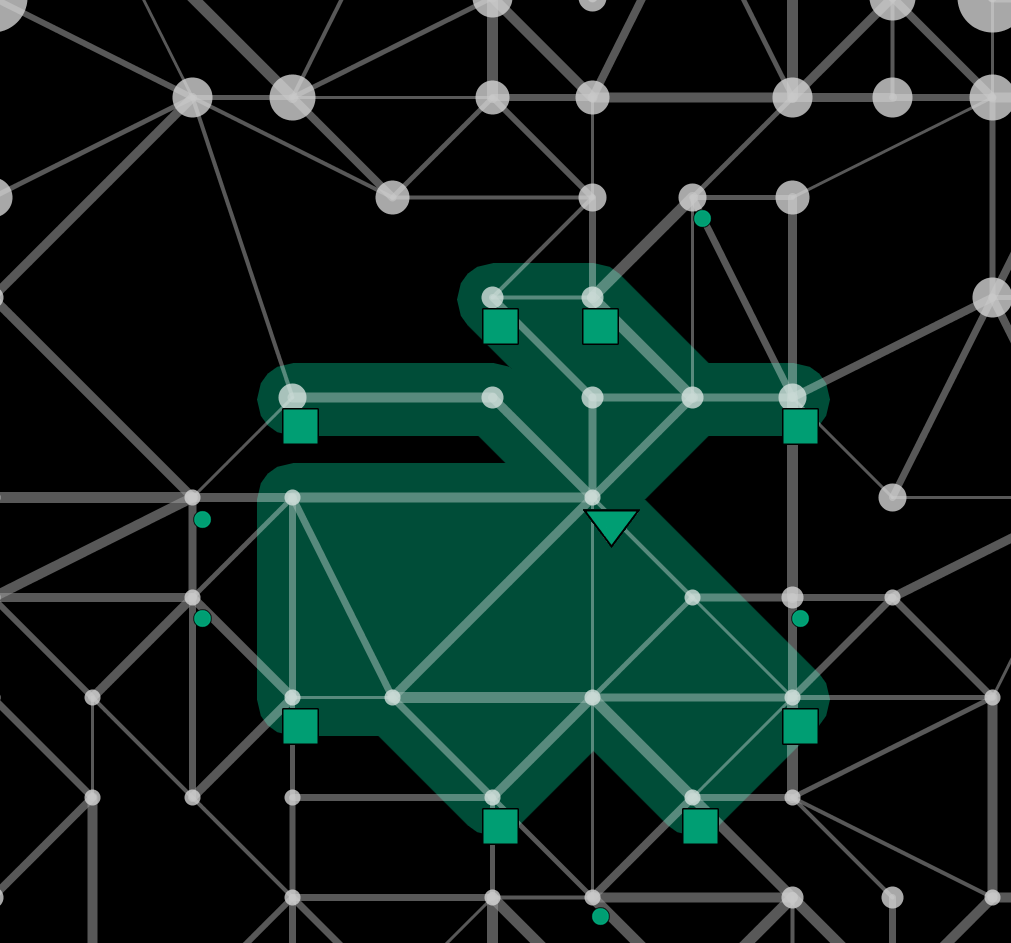
\includegraphics[width=.49\linewidth]{images/zone4.png}}
  \caption{Four examples of zones calculated by the heuristic algorithm described in \autoref{alg:zon_calculation}. The green squares and triangles represent the placement of agents, where the triangle is the agent on the center node. Nodes marked with a small green circle are optional agent positions that can be used to expand the zone if there are agents left over at the end of the zone building, as described in \autoref{alg:zon_finding}. The green-colored area represents the zone that is established by the given agent placement.}
  \label{fig:zones}
\end{figure}
blah
\iffalse % comments out the following
Due to the way the server-side colouring algorithm works, placing $N$ agents on the map so that they establish the highest possible zone value per step is anything but straight-forward. Even for $n = 1$, a single agent placed on an articulation point in the graph can establish a high-value zone if there are no enemy agents in either subgraph that it splits the map into. \autoref{fig:articulation_points} shows an example.
\begin{figure}
  \centering
  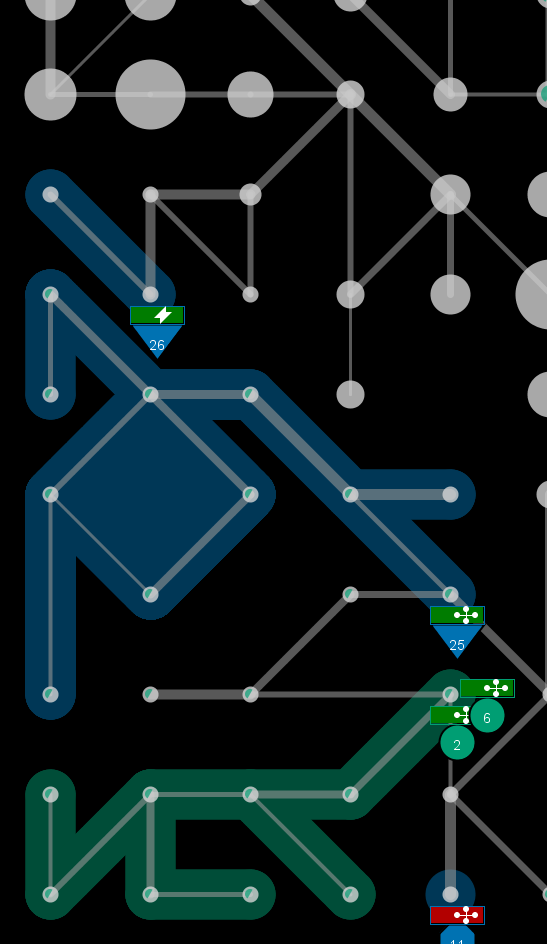
\includegraphics[width=\gri\textwidth]{articulation_points}
  \caption{The control loop for the agent deliberation process in the BOID architecture. Taken from \citeauthor{broersen2002goal}~\cite{broersen2002goal}.}
  \label{fig:control}
\end{figure}
In some way, we try to find local maxima to build small zones with as few agents as possible. How do we find zones? How do we find out how many agents we need? Explain that extending zones describes how the score resulting from an active zone can be increased by using idle agents. How do we determine what additional spots for zone extensions exist?
Present our colouring algorithm and the concept of a centre node.
\fi
